\documentclass[12pt,a4paper]{article}

%=============================================================================
% CONFIGURACIÓN DE FORMATO BAJO NORMAS APA 7ma EDICIÓN (RIGUROSO)
%=============================================================================

%-----------------------------------------------------------------------------
% DISEÑO DE PÁGINA Y MÁRGENES (APA 7: 1 pulgada o 2.54 cm en los 4 lados)
%-----------------------------------------------------------------------------
\usepackage[a4paper, margin=2.54cm]{geometry}

%-----------------------------------------------------------------------------
% NUMERACIÓN DE PÁGINAS Y ENCABEZADOS (Solución al problema de la esquina superior)
%-----------------------------------------------------------------------------
\usepackage{fancyhdr}
\pagestyle{fancy}
\fancyhf{} % Borra por completo encabezados y pies de página anteriores

% Configura el número de página estrictamente en la esquina superior derecha
\rhead{\thepage} 
\lhead{}  % En trabajos estudiantiles NO se usa encabezado de texto (Running Head)
\cfoot{}  % Garantiza que no quede ningún número flotando abajo al centro

% Elimina las líneas horizontales decorativas del encabezado y pie (Prohibidas en APA)
\renewcommand{\headrulewidth}{0pt}
\renewcommand{\footrulewidth}{0pt}

% REDEFINICIÓN CRÍTICA DEL ESTILO 'PLAIN'
% Evita que LaTeX mueva el número abajo en el índice o inicios de sección
\fancypagestyle{plain}{
	\fancyhf{}
	\rhead{\thepage}
	\renewcommand{\headrulewidth}{0pt}
	\renewcommand{\footrulewidth}{0pt}
}

%-----------------------------------------------------------------------------
% INTERLINEADO Y SANGRÍAS
%-----------------------------------------------------------------------------
\usepackage{setspace}
\doublespacing % APA 7 exige doble espacio reglamentario en todo el texto, tablas y notas
\setlength{\parindent}{1.27cm} % Sangría reglamentaria de 0.5 pulgadas (1.27 cm)

%-----------------------------------------------------------------------------
% IDIOMA Y TRADUCCIÓN
%-----------------------------------------------------------------------------
\usepackage[spanish, es-tabla]{babel} % 'es-tabla' evita que LaTeX escriba "Cuadro" en vez de "Tabla"

%-----------------------------------------------------------------------------
% FUENTES Y MATEMÁTICAS
%-----------------------------------------------------------------------------
\usepackage[T1]{fontenc}
\usepackage[utf8]{inputenc}
\usepackage{amsmath, amsfonts, amssymb, bm, mathtools}

%-----------------------------------------------------------------------------
% JERARQUÍA DE TÍTULO / ENCABEZADOS (NIVELES APA 7)
%-----------------------------------------------------------------------------
\usepackage{titlesec}

% Nota institucional: APA puro no numera los títulos. Como en ingeniería de la UNT 
% se exige numeración decimal (1., 1.1), se conserva el formato numérico pero adaptado 
% visualmente a la posición y estilo estricto de APA 7.

% Nivel 1 (\section): Centrado, Negrita
\titleformat{\section}[block]
{\normalfont\large\bfseries\centering}{\thesection.}{1em}{}

% Nivel 2 (\subsection): Alineado a la izquierda, Negrita
\titleformat{\subsection}[block]
{\normalfont\normalsize\bfseries}{\thesubsection.}{1em}{}

% Nivel 3 (\subsubsection): Alineado a la izquierda, Negrita, Cursiva
\titleformat{\subsubsection}[block]
{\normalfont\normalsize\bfseries\itshape}{\thesubsubsection.}{1em}{}

% Nivel 4 (\paragraph): Con sangría, Negrita, punto al final, texto continuo en la misma línea
\titleformat{\paragraph}[runin]
{\normalfont\normalsize\bfseries}{\theparagraph.}{1em}{}[.]
\titlespacing*{\paragraph}{\parindent}{1.5ex plus 0.5ex minus 0.2ex}{1em}

% Nivel 5 (\subparagraph): Con sangría, Negrita, Cursiva, punto al final, texto continuo en la misma línea
\titleformat{\subparagraph}[runin]
{\normalfont\normalsize\bfseries\itshape}{\thesubparagraph.}{1em}{}[.]
\titlespacing*{\subparagraph}{\parindent}{1.5ex plus 0.5ex minus 0.2ex}{1em}

%-----------------------------------------------------------------------------
% TABLAS Y FIGURAS AUTOMATIZADAS (ESTILO APA 7)
%-----------------------------------------------------------------------------
\usepackage{graphicx}
\usepackage{longtable}
\usepackage{array}
\usepackage{booktabs} % Indispensable para tablas APA (elimina líneas verticales)
\usepackage{float}
\usepackage{caption}

% Automatización completa de los Captions:
% El número ("Tabla 1") saldrá en NEGRITA. El título descriptivo irá ABAJO en una nueva línea y en CURSIVA.
\captionsetup{
	labelsep=newline,          % Envía el título a una línea nueva
	justification=raggedright, % Alineado a la izquierda
	singlelinecheck=false,     % Evita que captions cortos se centren solos
	labelfont=bf,              % Etiqueta en Negrita
	textfont=it                % Texto del título en Cursiva
}

%-----------------------------------------------------------------------------
% OTROS PAQUETES DE TU PROYECTO
%-----------------------------------------------------------------------------
\usepackage{pdfpages}
\usepackage{tocloft}
\usepackage{tikz}
\usepackage[dvipsnames]{xcolor}

%-----------------------------------------------------------------------------
% HIPERVÍNCULOS
%-----------------------------------------------------------------------------
\usepackage[breaklinks]{hyperref}
\hypersetup{
	colorlinks=true,
	linkcolor=black,
	filecolor=black,      
	urlcolor=blue,
	citecolor=black
}

\begin{document}
	
	% CARATULA
	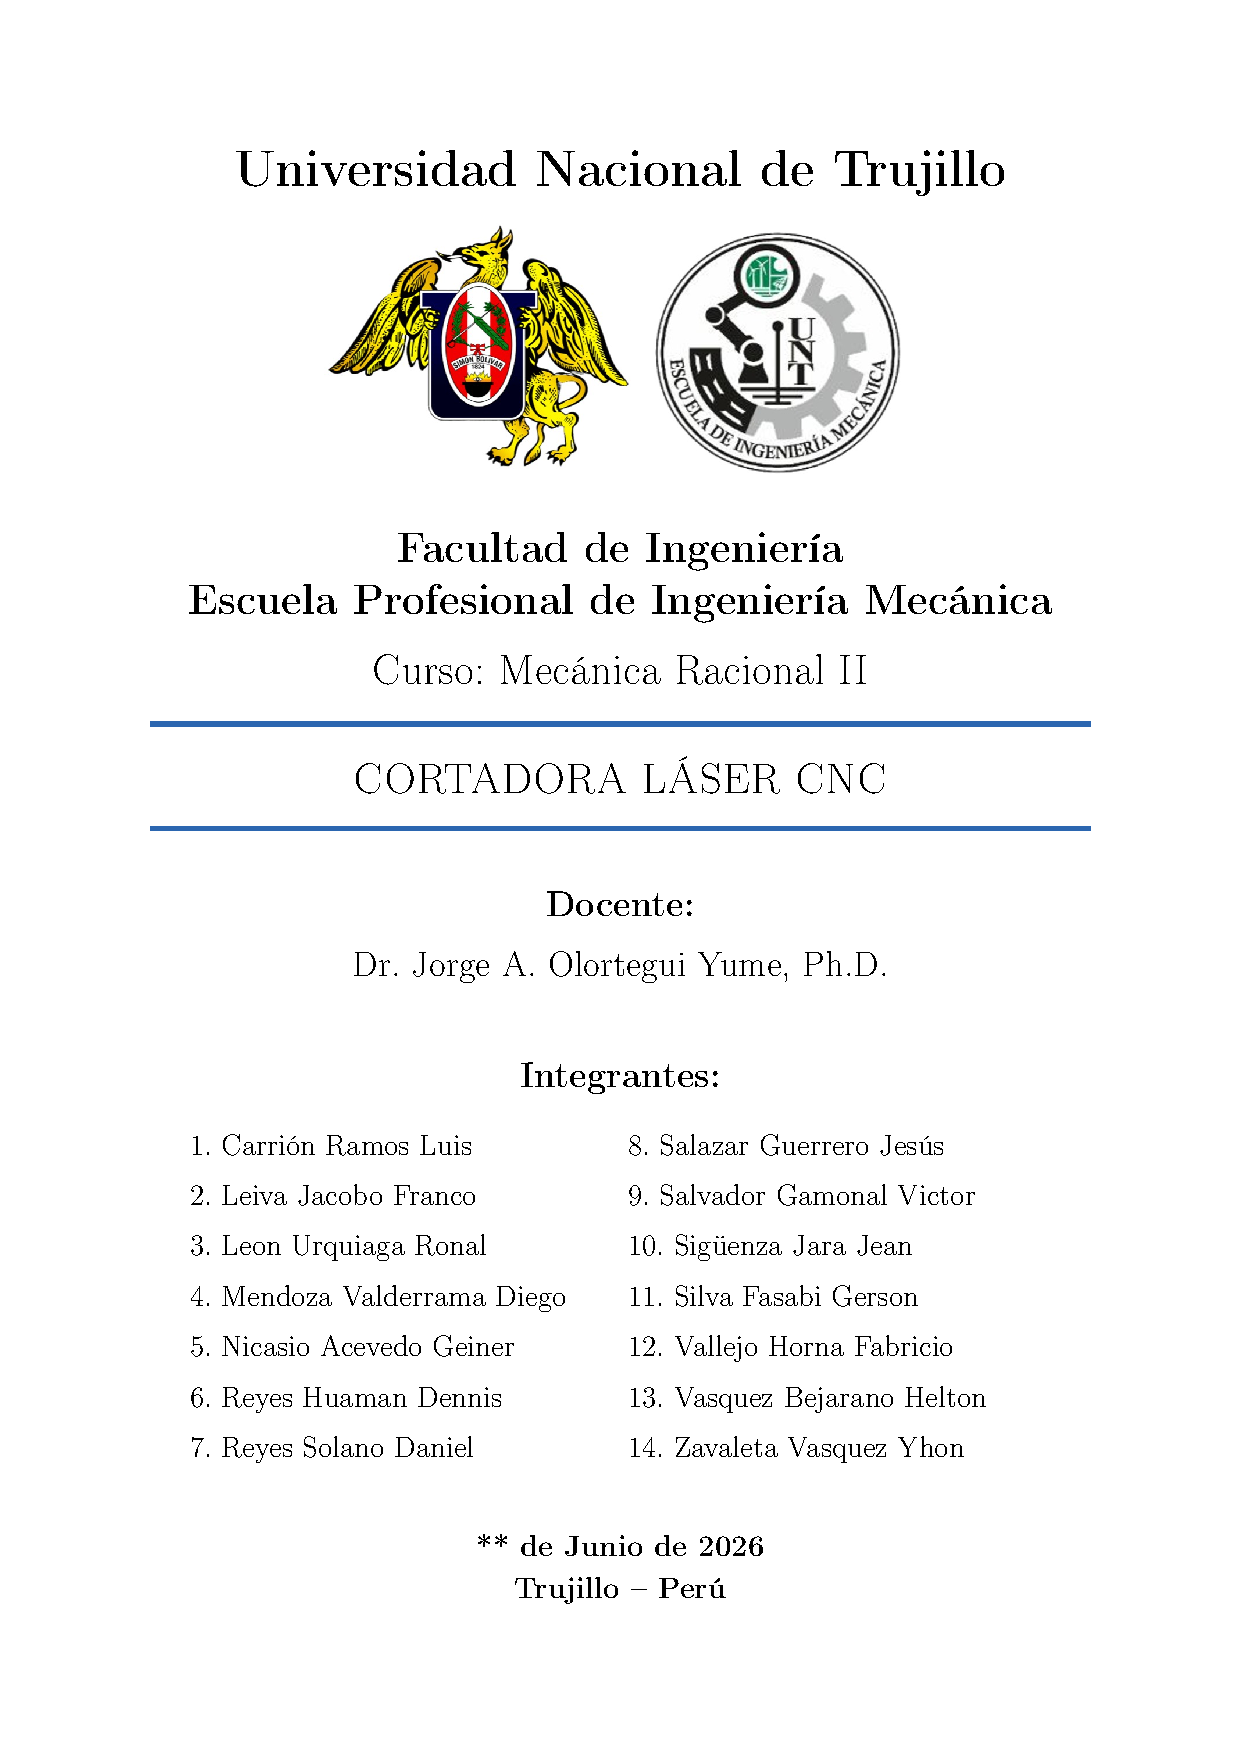
\includepdf[pages=-]{CARATULA/CARATULA.pdf}
	
	% INDICE
	\tableofcontents
	
	% CUERPO
	
	%------------------------------------------------
	
	% CAPITULO 1
	
	\section{INTRODUCCIÓN}

\subsection{Importancia del Modelado y Simulación de \ldots}

\subsection{Trabajos previos en Modelado y Simulación Dinámica de \ldots}

\subsection{Planteamiento del Problema a resolver}

\subsection{Objetivos}

\begin{table}[htbp]
	\caption{Propiedades mecánicas del aluminio 6061-T6} % Solo escribe el título normal
	\label{tab:propiedades}
	\centering
	\begin{tabular}{lcc}
		\toprule % Línea superior
		Propiedad & Valor & Unidad \\
		\midrule % Línea debajo de los encabezados
		Módulo de elasticidad & 68.9 & GPa \\
		Límite de fluencia & 276 & MPa \\
		Resistencia última & 310 & MPa \\
		Densidad & 2700 & kg/m$^3$ \\
		\bottomrule % Línea inferior final
	\end{tabular}
	\vspace{0.2cm}
	
	\raggedright % La nota va alineada a la izquierda
	\textit{Nota.} Datos obtenidos de Callister y Rethwisch (2020).
\end{table}

\begin{figure}[htbp]
	\caption{Modelo CAD de la cortadora láser CNC}
	\label{fig:cad}
	\centering
	\includegraphics[width=0.8\textwidth]{example-image-a}
	\vspace{0.2cm}
	
	\raggedright
	\textit{Nota.} Diseño preliminar del equipo ensamblado.
\end{figure}
	
	% CAPITULO 2
	
	\section{FUNDAMENTO TEÓRICO}

\subsection{Máquinas CNC}

\subsection{Historia de las Máquinas CNC}

\subsection{El Código G}

\subsection{Software para la simulación del proceso de \ldots}

\subsection{Partes de una Máquina CNC}

\subsection{Normativa relacionada con Máquinas CNC}

\subsubsection{Norma UNE \ldots}

\subsubsection{Norma ASTM \ldots}

\subsubsection{Estándar ASME \ldots}

\subsection{Generalidades de la Cinemática y Cinética del Maquinado en Máquinas CNC}

\subsection{Descripción de la máquina o sistema electromecánico}

\subsection{Principios de conversión de energía}

\subsubsection{Torque, potencia, velocidad}

\subsubsection{Eficiencia y pérdidas}

\subsubsection{Campo magnético e inducción}

\subsubsection{Régimen de operación y curva característica}

\subsubsection{Especificaciones de ingeniería}

\paragraph{Requerimientos funcionales}

\paragraph{Requerimientos eléctricos}

\paragraph{Requerimientos mecánicos}

\paragraph{Seguridad, Operación y Ambiente de trabajo}

\paragraph{Normas básicas y criterios de aceptación}
	
	% CAPITULO 3
	
	\section{MODELADO ANALÍTICO DE LA DINÁMICA DEL MAQUINADO CNC}

\subsection{Modelo Analítico de la Cinemática 3D del proceso de fabricación maquinado con CNC de un impulsor de turbina (o impulsor de bomba, o propulsor, o engranaje cónico helicoidal)}

\subsubsection{\ldots}

\subsubsection{\ldots}

\subsubsection{\ldots}

\subsection{Modelo Analítico de la Cinética 3D del proceso de fabricación maquinado con CNC de un impulsor de turbina (o impulsor de bomba, o propulsor, o engranaje cónico helicoidal)}

\subsubsection{\ldots}

\subsubsection{\ldots}

\subsubsection{\ldots}
	
	% CAPITULO 4
	
	\section{APLICACIÓN DE LOS MODELOS CINEMÁTICOS Y CINÉTICOS}

\subsection{Cálculo de \ldots}

\subsubsection{XXXXX}

\subsubsection{XXXXX}

\subsubsection{XXXXX}

\subsubsection{XXXXX}

\subsection{Programa MATLAB para el ANÁLISIS CINEMÁTICO y CINÉTICO}

\subsection{Interface Gráfica de Usuario (GUI) para el ANÁLISIS CINEMÁTICO y CINÉTICO}
	
	% CAPITULO 5
	
	\section{RESUMEN DE RESULTADOS}

\subsection{Posiciones}

\subsection{Velocidades}

\subsection{Aceleraciones}

\subsection{Fuerzas y Momentos}

\subsection{Potencias}

\subsection{Diagrama de \ldots}

	
	% CAPITULO 6
	
	\section{ELABORACIÓN DE PLANOS}

\subsection{Selección de Componentes}

\subsection{Plano General}

\subsection{Planos de Detalle o Despieces}

\subsection{Plano de Ensamble o Explotado}

\subsection{Diagramas de fuerza, mando y conexión}

\subsection{Diagramas de Montaje}

\subsection{Diagramas de Estructura}

\subsection{Diagramas de Transmisión mecánica}

\subsection{Diagramas de Gabinete, protecciones y secuencia de operación}
	
	% CAPITULO 7
	
	\section{PROCESO DE FABRICACIÓN}

\subsection{Materiales}

\subsection{Herramientas}

\subsection{Equipos}

\subsection{Ensamble}
	
	% CAPITULO 8
	
	\section{PRUEBAS, MEDICIONES Y VALIDACIÓN EXPERIMENTAL}

\subsection{Protocolo de Pruebas}

\subsection{Instrumentos de Medición}

\subsection{Tablas de Datos}

\subsection{Cálculos de Potencia y Eficiencia Experimentales}

\subsection{Comparación con Valores Teóricos Calculados}
	
	% CAPITULO 9
	
	\section{SEGURIDAD, MANTENIMIENTO Y SOSTENIBILIDAD}

\subsection{Seguridad eléctrica}

\subsection{Seguridad mecánica}

\subsection{Protección del usuario}

\subsection{Mantenimiento preventivo}

\subsection{Eficiencia energética}

\subsection{Recomendaciones de operación}
	
	% CAPITULO 10
	
	\section{ANÁLISIS ECONÓMICO}

\subsection{Listado de Componentes}

\subsection{Presupuesto}
	
	% CAPITULO 11
	
	\section{ARCHIVO GRÁFICO}

\subsection{XXXXX}

\subsection{XXXXX}

\subsection{XXXXX}

\subsection{XXXXX}
	
	% CAPITULO 12
	
	\input{CAPITULO_12_CONCLUSIONES Y RECOMENDACIONES/CONCLUSIONES}
	
	\section*{REFERENCIAS}
	\addcontentsline{toc}{section}{REFERENCIAS}
	
	% ANEXOS
	
	\section{Evaluación de cumplimiento de integrantes de grupo}

\section{Avance No 00}

\section{\ldots}

\section{\ldots}

\section{Catálogo \ldots}

\section{Tabla \ldots}

\section{Gráfica \ldots}

\section{Gráfica \ldots}

\section{\ldots}

\section{\ldots}

\section{Limpieza y Ordenamiento Final del Laboratorio}

\section{Ficha Técnica de Fresa de espiga de Punta redondeada de 3 mm en HSS -- Acabado}

\section{Ficha Técnica de Fresa de espiga de 6 mm en HSS -- Desbaste}

\section{Ficha Técnica de Fresa de espiga de 10 mm en HSS -- Desbaste}

\section{Plano General}

\section{Plano de Detalle (Despiece)}

\section{Plano en Vista Explotada}

\section{Ficha Técnica de Motor XYZ 34-Z (Ejemplo)}
	
	\appendix
	
\end{document}